%!TEX encoding = UTF-8 Unicode
%!TEX program = xelatex

\documentclass[bachelor]{ustcthesis}
% bachelor|master|doctor
\usepackage{ustcextra}
\graphicspath{{figures/}}
\bibliographystyle{ustcauthoryear}
% \bibliographystyle{ustcnumerical}

\title{中国科学技术大学\\中文知识关系抽取的研究与实现}
\author{曾锃煜}
\major{计算机科学与技术}
\advisor{陈欢欢\ 教授}
\submitdate{二〇一七年六月}
%\secrettext{机密\quad 小于等于20年}   % 内部|秘密|机密,注释本行则不保密
\depart{十一系}

\entitle{Research and Realization of Chinese Knowledge Relation Extraction}
\enauthor{Zengyu Zeng}
\enmajor{Computer Science and Tech.}
\enadvisor{Prof. Huanhuan Chen}
\ensubmitdate{June, 2017}
%\ensecrettext{Confidential\quad Less than or equal to 20 years}  % Internal|Secret|Confidential

\begin{document}

\maketitle

%
% 本科论文:
%   frontmatter: 致谢、目录、中文摘要、英文摘要
%   mainmatter: 正文章节、参考文献
%   appendix: 附录
%
% 硕博论文:
%   frontmatter: 中文摘要、英文摘要、目录、符号说明
%   mainmatter: 正文、参考文献
%   appendix: 附录
%   backmatter: 致谢、发表论文
%

\frontmatter
\begin{acknowledgements}

在中国科技大学完成本科学业的四年里,我所从事的学习和研究工作,都是在导师以及系里其他老师和同学的指导和帮助下进行的。在完成论文之际,请容许我对他们表达诚挚的谢意。

感谢班主任王海龙老师多年的关怀。感谢陈欢欢、蒋凡等老师,他们本科生阶段的指导给我现在的研究工作打下了基础。

感谢张练钢等师兄师姐们的指点和照顾;感谢李卓华等几位同班同学,与你们的讨论使我受益良多;感谢王译锋等师弟师妹,我们在实验室共同学习共同生活,一起走过了这段愉快而难忘的岁月。

感谢科大,感谢一路走过来的兄弟姐妹们,在最宝贵年华里,是你们伴随着我的成长。

最后,感谢我家人一贯的鼓励和支持,你们是我追求学业的坚强后盾。

\vskip 18pt

\begin{flushright}

曾锃煜

\today

\end{flushright}
\end{acknowledgements}

\tableofcontents
\listoffigures
\listoftables
\listofalgorithms  % 算法索引,如不需要,可直接注释掉本行
\begin{abstract}
互联网不断发展,其中的信息也随着时间日渐增多,传统的返回检索方式开始无法满足获取所需信息和知识资源的全面性和以高效率完成。实体的知识关系抽取,可以从自然语言(中文文本)中抽取实体,并将实体之间的关系结构化,提高了用户可获取信息的全面性和获取的效率。

信息提取(IE)系统寻求从自然语言中提取语义关系文本,但大多数系统使用监督学习关系特定的例子,因此受到训练数据可用性的限制。开放式信息提取系统例如 TextRunner,在另一方面,致力于处理没有限制数量的从互联网获取的实体关系。

传统上,信息提取专注于精确、狭义的、预先指定的要求。例如从一些会议通告里提取时间和地点。而转移到另一个领域里,则需要用户对实体关系命名并手工制定新的提取规则或对新的训练集例子进行手工标注。这样的人力工作量随着目标实体关系的数量线性增加。

开放式关系抽取(Open Relation Extraction,ORE)是实体关系抽取的一种,它克服了传统信息提取(IE)的缺陷,即传统的信息获取技术对每种关系模式各自训练了他们的提取器。

有很多系统流行于英文的 ORE,例如 OLLIE,ReVerb 和 Exemplar 等。然而,对于其他语言的 ORE 则基本没有相关研究的报告。本毕业设计采用了基于语法分析的系统 ZORE(Zh ORE)来对简体中文文本进行关系和语义模式的抽取。ZORE 从自动解析的依赖树里定义了候选的关系,然后将实体的关系和语义模式不断地通过一种新的双重传播算法。

本文内容包括了对于所采取的实体关系抽取系统(ZORE)的介绍及其实现,以及关于 ZORE 所需组件的介绍,并将其应用在实际工程中。

\keywords{开放式关系抽取\zhspace{} ZORE\zhspace{} 双重传播算法}
\end{abstract}

\begin{enabstract}
With the continuous development of the Internet, with the passage of time, more and more information, the traditional return search method began to meet the need to obtain the required information and knowledge resources needs, fully and effectively completed. The knowledge of the entity can be extracted from the natural language (Chinese text), the structure of the relationship between the entities, and improve the user's available information is comprehensive and efficient.

The information extraction (IE) system seeks to extract semantic relations text from natural language, but most systems use specific examples of supervised learning relationships, thus limiting the availability of training data. On the other hand, an open information extraction system such as TextRunner is dedicated to handling unrestricted physical relationships obtained from the Internet.

Traditionally, information extraction focuses on precise, narrow and pre-defined requirements. Such as extracting time and place from certain meeting notifications. And move to another domain, the user needs to name the entity relationship and manually create a new extraction rule or manually annotate the new training set example. The human workload increases linearly with the number of target entities.

Open relational extraction (ORE) is an entity relationship extraction that overcomes the shortcomings of traditional information extraction (IE), the traditional information acquisition techniques for each relational model to develop their extractors.

English ORE has many popular systems, such as OLLIE, ReVerb and Exemplar. However, ORE in other languages ​​is basically no relevant research report. The graduation design uses a system based on parsing. ZORE (Zh ORE) simplifies the relationship between Chinese text and semantic models. Zore defines the candidate relationship from the automatic resolution dependency tree, and then passes the entity's relationship and semantic pattern continually through the new dual-propagation algorithm.

This article introduces the introduction and implementation of the Entity Relationship Extraction System (ZORE), and introduces the components required by ZORE and applies it to the actual project.

\enkeywords{Open relation extratction, ZORE, Double propagation algorithm}
\end{enabstract}



\mainmatter
\chapter{绪论}
\label{chap:introduction}

本章的内容包括实体关系知识抽取的研究背景与其意义,阐释了在当先信息大爆炸的时代里,如何从不计其数的信息中提取出实体,之后从实体之间抽取出关系元组来建立全面而准确的信息知识数据库,从而更好地服务互联网的使用者。也介绍了国内外对于本课题的研究现状和本文的研究内容,以及概述中文开放式关系抽取系统中所使用的机器学习算法。

\section{研究背景与意义}

\subsection{研究背景}

传统的信息提取涉及很多人为因素的干扰,包括以手工制定的规则或手工标注出来的样例来作为机器学习的预定义参数,之后才能识别并判断在输入的文本中两个实体之间的特定关系\citep{wang}。即使机器学习可以帮助枚举出潜在的可供提取的关系模式,但这个方式常常只能提取已经被预定义的关系集。并且,这个方式不适用于如今的互联网,因为其当中的信息大都是非结构化、未预先定义实体关系的。

另一种开放的信息抽取\citep{banko}方式则不需要人工对每种关系类型进行预定义,它可以从文本抽取关系并能方便地度量网络语料库的多样性和覆盖范围。语料库是开放式信息抽取系统所需要的唯一一种输入数据,它的输出则是被抽取出的各种关系的集合。一个开放式信息抽取系统通过它的语料库大小来控制它所能抽取关系的可扩展性,并用以下方法来增加可处理的关系类型:基于浅分析、基于语法或没有预定义关系的基于词法分析的模式匹配\citep{wu2010, naka2012, etz2011}。现在的开放式关系抽取技术关注于字面上关系的抽取,而没有尝试进行词法分析,但词法分析却是传统信息抽取的优点。

\subsection{研究意义}
中文开放式关系抽取外的其他的开放式关系抽取系统是抽取二元的关系,之后将其归纳为语义模式。而中文开放式关系抽取则同时进行抽取关系和归纳模式,利用双重拓展的算法让关系和模式信息互相加固加强,从而减弱自动词法分析和自动语义分析所带来的负面影响,语义模式信息可以帮助提升关系抽取的质量。所以本次毕设采用了中文开放式关系抽取做为关系抽取的引擎。

\section{开放式关系抽取的基本定义}
中文开放式关系抽取被应用于网络文本来提取普遍意义上的关系和它们的语义类型。对于关系的定义大部分都是来自于英文语境下,但是此次毕设的语义环境处在中文里,所以需要对基于英文语境下的开放式关系抽取进行一些适合中文语境的调整。以下的概念定义以句子“侯建国校长就职于中国科学技术大学。”做为样例。

\begin{figure}[ht]
\centering
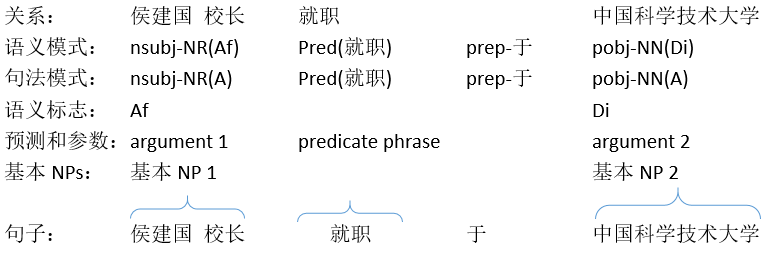
\includegraphics[width=15cm]{sentence1}
\caption{分析样例句子}\label{fig:sentence1}
\end{figure}

\subsection{谓词短语(predicate phrase)}
谓词短语是包括至少一个动词或系词,并在语句构成上控制至少一个名词的词语序列。例如,图 ~\ref{fig:sentence1} 里的谓词短语是“就职”。为了预防“少动词结构”的情况出现,动词和它所直接“控制”的对象共同被认为是一个“谓词短语”。介词并不被包括在谓词短语的范围中。

\subsection{论元(argument)}
论元是一个被谓词短语所直接控制或通过介词间接控制的基本名词短语。例如,图 ~\ref{fig:sentence1} 里的“侯建国校长”和“中国科学技术大学”就是谓词短语“就职”的两个论元。

\subsection{关系(relation)}
一个“二元关系”是一个包括了谓词短语 pred 和它的两个论元 x 与 y 的三元组。依此类推,一个“n 元关系”则包括了 n 个论元。例如,图 ~\ref{fig:sentence1} 里的句子包含了一个二元关系(x[侯建国校长], pred[就职], y[中国科学技术大学])。在英文语境下,二元关系的两个论元通常分别位于 pred 的左边和右边。因此,弱模式对于英文语境下的的关系抽取非常有效。然而在中文语境下,二元关系的两个关系有可能都在 pred 的左边(例如“我和你打架”),都在 pred 的右边(例如“抄袭了我的作业”),或者一左一右分布在 pred 的两边,即根据不同的句子,出现的关系模式可能为(x, y, pred),(pred, x, y)和(x, pred, y)。从而让关系短语的探测变得更加复杂。

\subsection{句法模式(syntactic pattern)}
句法模式是一个关系的句法抽象,一个关系可以被推广到字词的组合、POS 标签(Part of speech,词性标注标签)和句法依赖标志。例如,图 ~\ref{fig:sentence1} 中的句法模式是\{nsubj-NR(A), Pred[就职], prep-于, pobj-NN(A)\}。它由四个子模式组成。第一个子模式 nsubj-NR(A) 表示当前的短语扮演着具有 POS 标签 NR (proper nouns,专有名词)的谓词短语的主语,在这里(A)意味着这个短语是被提取出的关系中的论元。第二个子模式表示图 ~\ref{fig:sentence1} 中的样例句子谓词短语是“就职”。并且在谓词和论元中的字词(例如 prep-于)被直接包括在模式中。

\subsection{语义标志(semantic signature)}
一个关系里的语义标志包括着论元的语义分类。图 ~\ref{fig:sentence1} 中的语义标志是(Af, Di),其中 Af 表示“人类”,Di 表示“院校”。

\subsection{语义模式(semantic pattern)}
语义模式是一个关系里的语义抽象。它是由句法模式和语义标志结合成的。例如,句法模式\{nsubj-NR(A), Pred[就职], prep-于, pobj-NN(A)\}与语义标志(Af,Di)结合,就生成了语义模式{nsubj-NR(Af), Pred[就职], prep-于, pobj-NN(Di)}。

\section{机器学习相关算法}
\subsection{聚类}
\subsubsection{基本概念}
聚类即将实体根据他们之间具有的属性进行处理,有相似属性的则聚集为一个类别,使得聚集出的同一种类别内部的所有实体之间都具有较高的相似性,而不是属于同一种类别的实体之间的相似性则较低。对聚类算法的度量主要是度量其使用的计算相似性和距离的方法。

对实体进行聚类,需要对不同实体之间的相似度和距离进行计算。即两个实体之间的距离越近,则他们的相似度就越高,也就是由更高的可能性被归类到同一个类别中。常见的距离和相似度计算度量类别较多,将结合公式在下文进行介绍,以两个 m 维向量 $X = (x_1, x_2 ......, x_m)$ 和 $Y = (y_1, y_2 ......, y_m)$ 表示两个实体之间的相似度和距离计算公式, $S_{ij}$ 和 $D_{ij}$ 分别代表两个向量之间的相似度和距离。
\newtheorem*{oujilide}{欧几里得距离}
\begin{oujilide}
    \begin{equation}
        d_{ij}(X,Y) = \sqrt{\sum_{k=1}^m|{x_k - y_k}|^2}
    \end{equation}
\end{oujilide}

\newtheorem*{yuxian}{余弦相似度}
\begin{yuxian}
    \begin{equation}
        S_{ij}(X, Y) = cos(\theta) = \frac{\sum_{k=1}^mx_ky_k}{\sqrt{\sum_{k=1}^mx_k^2}\sqrt{\sum_{k=1}^my_k^2}}
    \end{equation}
\end{yuxian}

\newtheorem*{manhadun}{曼哈顿距离}
\begin{manhadun}
    \begin{equation}
        d_{ij}(X,Y) = \sum_{k=1}^m|x_k-y_k|
    \end{equation}
\end{manhadun}

\newtheorem*{qiebixuefu}{切比雪夫距离}
\begin{qiebixuefu}
    \begin{equation}
        d_{ij}(X,Y) = \max \limits_{1 \leq k \leq m}|x_k - y_k|
    \end{equation}
\end{qiebixuefu}

\newtheorem*{xiangguanxishu}{相关系数}
\begin{xiangguanxishu}
    \begin{equation}
        d_{ij}(X,Y) = \frac{\sum_{k=1}^m(x_k-\overline{X})(y_k-\overline{Y})}{\sqrt{\sum_{k=1}^m(x_k-\overline{X})}\sqrt{\sum_{k=1}^m(y_k-\overline{Y})}}
    \end{equation}
\end{xiangguanxishu}

\newtheorem*{mingkefusiji}{名科夫斯基距离}
\begin{mingkefusiji}
    \begin{equation}
        d_{ij}(X,Y) = \left( \sum_{k=1}^m|x_k-y_k|^q \right) ^ \frac{1}{q}, q > 0
    \end{equation}
\end{mingkefusiji}

若名氏距离里的 $q=0$ 则为曼哈顿距离,$q=1$ 则为欧几里得距离,$q\to \infty$ 则为切比雪夫距离。

\subsubsection{几种不同的聚类方法}
因为互联网数据的类别和数量都很多,所以目前没有一个普适的聚类算法可以用来对每种类型的数据进行梳理。需要使用算法处理特定类型的数据时,应该考虑待处理数据的特点、聚类的目的及使用场景。如图 ~\ref{fig:cluster}。

\begin{figure}[ht]
\centering
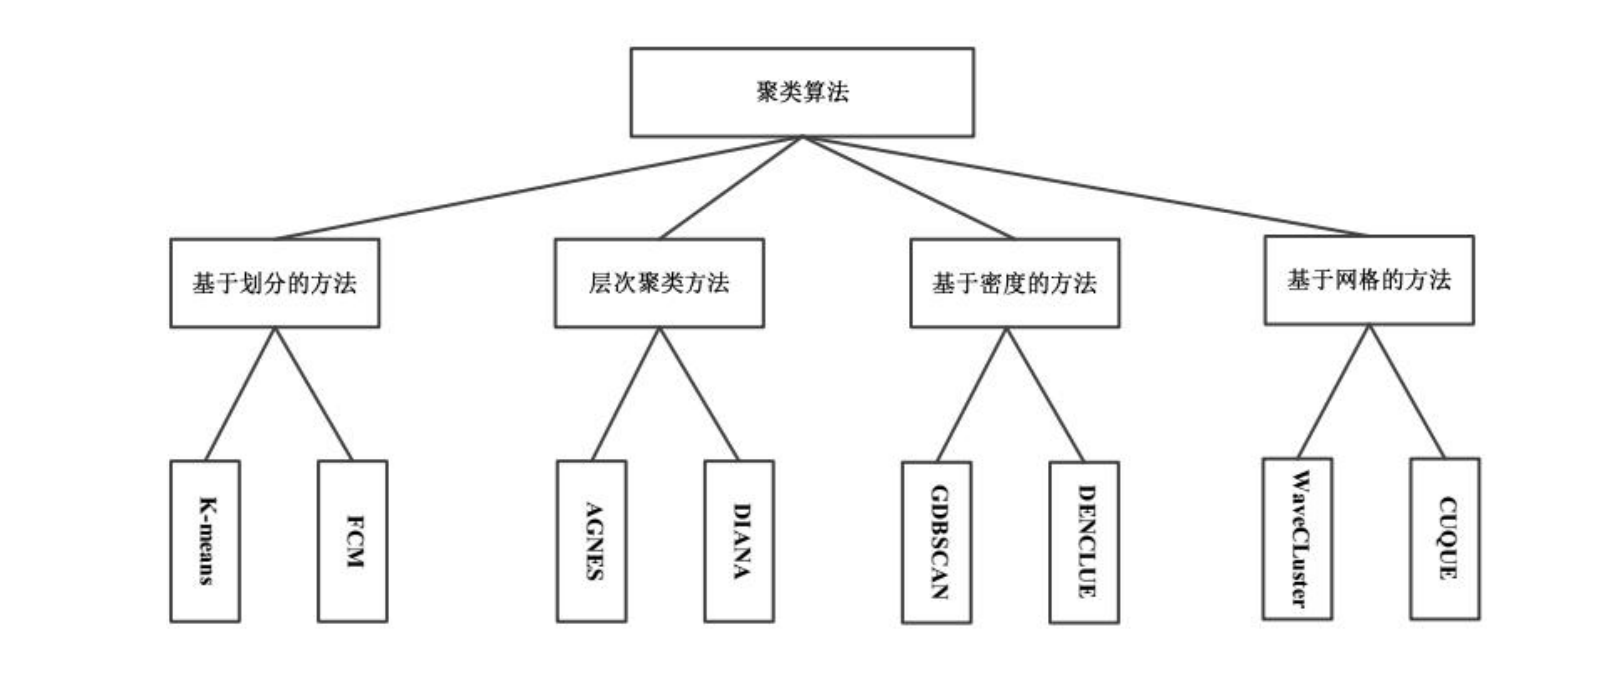
\includegraphics[width=13cm]{cluster}
\caption{聚类算法的归类}\label{fig:cluster}
\end{figure}

\newtheorem*{huafenfa}{基于划分的方法}
\begin{huafenfa}
    该方法为把有 n 个元素的数据集分割成 k 个子集,$k \leq n$。而划分结果中的每一个子集就是一个类别,也就是聚类之后的一个簇。而 K-means 算法,即是最经典的基于划分的聚类方法。
\end{huafenfa}

\newtheorem*{cengcijuleifa}{层次聚类方法}
\begin{cengcijuleifa}
    这个方法是将数据集以逐层进行的方法来处理,方向有自下而上,也有自上而下。而两个方向则分别是合并小类别(凝聚层级聚类)与将大类别分割(分裂层次聚类)。凝聚层次聚类就是对每种小类别进行迭代地合并直至达到结束条件,而算法初始时,将数据集的每个元素都视为一个类别,该聚类方法的典型算法是 $AGNES$ 算法。分裂层次聚类则与凝聚层次聚类相反,是对每种类别进行迭代地分割,直至达到算法结束条件,算法初始下,将整个数据集视为一个类别,这种方法的典型算法则为 $DIANA$ 算法。
\end{cengcijuleifa}

\newtheorem*{midufa}{基于密度的方法}
\begin{midufa}
    该方法为依据所给的数据元素的密度,将其划分为不同的类别。即把数据元素组成的每个类别看成是散布在空间中的各自独立的区域。若数据集当中的邻接点达到了定下的阈值则停止聚类,否则继续进行,直至生成大量的类别。$GDBSCAN$,$DENCLUE$ 都是密度聚类的经典算法。
\end{midufa}

\newtheorem*{wanggefa}{基于网格的方法}
\begin{wanggefa}
    该方法为通过网格技术把所给的数据集分割为互相独立的网格结构,对在网格内部的数据采取聚类操作。这种方法的优势为聚类的时间复杂度与数据集内部的元素数无关,而是与网格数有关。而其性能则由划分的网格结构底层粒度决定,若粒度变细,则处理代价变大。对上层的单元分割时,统计信息网格并未将底层与其邻元的关系纳入考虑,所以这种方法时间复杂度虽然较低,但其生成的聚类结果精确性可能不尽如人意。$WaveCluster$,$CUQUE$ 都是经典的网格聚类算法。
\end{wanggefa}

\subsubsection{K-means 算法}
由之前的介绍我们已经知道,K-means 是一种经典的划分聚类算法,由数据之间的距离来度量其相似性,即距离越近,相似性越大。

算法 ~\ref{algo:kmeans} 的详细工作步骤为,第一步,随机生成 k 个点的坐标作为 k 个类别的起始中心坐标;第二步,对数据集内的每个元素都计算其与制定类别的起始中心距离,把当中样本的数据纳入离它最近的起始中心的类别的类,即得出了了起始的 k 个类别分布;第三步,接着对经过第二步处理的数据重新计算他们所属类别的中心坐标,之后执行与第二步相同的过程,若类别中心与之前的类别中心相同则算法结束,不然就接着重复第三步的过程,最后会得出收敛的 k 个类别的中心坐标。

\begin{algorithm}[!h]
\SetAlgoLined
\KwData{$n$ 个数据对象 $x_i$ 的集合 $X$}
\KwResult{$k$ 个聚类中心 $C_j$ 以及 $k$ 个类别的数据集合 $D_j$}
\SetKw{KwIns}{insert}
\SetKw{KwInt}{into}
\SetKw{KwT}{true}
\SetKw{KwF}{false}
    $flag = $\KwT \;
    initial $k$ protottype $C_j, j \in \left[ 1, k \right]$ \;
    \While{$flag$}{
        \For{$i \leftarrow 1$ \KwTo $n$}{
            $D\left( x_i, c_j \right) \leftarrow |x_i - c_j|$\;
        }
        \uIf{$D\left( x_i, c_j \right) = \min \{ D\left( x_i, c_j \right) \} $}{
            \KwIns $x_i$ \KwInt $D_j$\;
        }
        \uIf{$C_j$ changed}{
            $c_j \leftarrow \frac{1}{N} \sum_{p=1}^{N_j}x_{jp}, j \in 1,2, ......, k$\;
        }
        \Else{
            $flag =$ \KwF \;
        }
    }
\caption[K-means 算法]{K-means}
\label{algo:kmeans}
\end{algorithm}

\subsection{$Logistic$ 回归}
$Logistic$ 算法为一个经典的且应用广阔的机器学习算法。大致思想为通过计算得到的样本数据所属的每种类别的概率来推测其他样本所属的类别。

设想有一个训练数据集 $X$,其元素个数为 $n$ 个, $X = \{ x_1,x_2,......,x_n\}$,每个元素对应的类型标签 $Y=\{ y_1,y_2,......,y_n\}$,每个元素 $x_i$ 的维度是 $d$,形式是 $x=\left[ x^{\left( 1\right)},x^{\left( 2\right)},......,x^{\left( n\right)} \right] ^T, y \in \{ 1,2,......,c\}$。
\newtheorem*{yucehanshu}{预测函数}
\begin{yucehanshu}
    \begin{equation}
        h_{\theta}\left( x\right) =g\left( \theta^Tx\right) =\frac{1}{1+e^{-\theta^Tx}} \in \left[ 0,1 \right]
    \end{equation}
    其中的向量 $\theta$ 是需要学习的参数。
\end{yucehanshu}

\newtheorem*{sigmoid}{$Sigmoid$函数}
\begin{sigmoid}
    \begin{equation}
        g\left( z\right) =\frac{1}{1+e^{-z}} \in \left[ 0,1 \right]
    \end{equation}
\end{sigmoid}

而为了在实际使用中的便利性,令$x^{\left( 0 \right)} =1$,即 $\theta^Tx=\sum_{j=0}^d\theta_jx^{\left( j \right)}$。

算法的学习就是利用计算过程来获取 $\theta$,定义损失函数,之后以极大似然估计或最小化损失函数对 $\theta$ 进行计算。接下去以极大似然估计法来计算 $\theta$,假设 $X, Y$ 分别为样本集和其元素的归属类别集,二者互相独立,则每个样本的联合分布可由该样本的边际分布的乘积所求出。

\newtheorem*{jidasiran}{$\theta$ 的极大似然估计函数}
\begin{jidasiran}
    \begin{equation}
        L\left( \theta \right) = \prod_{i=1}^nP\left( y_i|x_i,\theta \right) = \prod_{i=1}^nh_{\theta}\left( x_i \right)^{y_i}\left(1-h_{\theta}\left(x_i \right) \right)^{1-y_i}
    \end{equation}
\end{jidasiran}

\newtheorem*{sunshihanshu}{损失函数}
\begin{sunshihanshu}
    \begin{equation}
        J\left( \theta \right) = -\frac{1}{n}\left( \sum_{i=1}^n\sum_{k=1}^nI\{ y_i=k\} log\frac{e^{\theta_k^Tx}}{\sum_{l=1}^ce^{\theta_l^Tx}} \right)
    \end{equation}

    当中 $I\{ y_i=k\}$ 即为指示器函数,如果 $y_i=k$ ,$I\{ y_i=k\} =1$,否则 $I\{ y_i=k\} =0$。
\end{sunshihanshu}

\chapter{相关技术背景及算法}
\label{chap:algorithm}

\begin{figure}[ht]
\centering
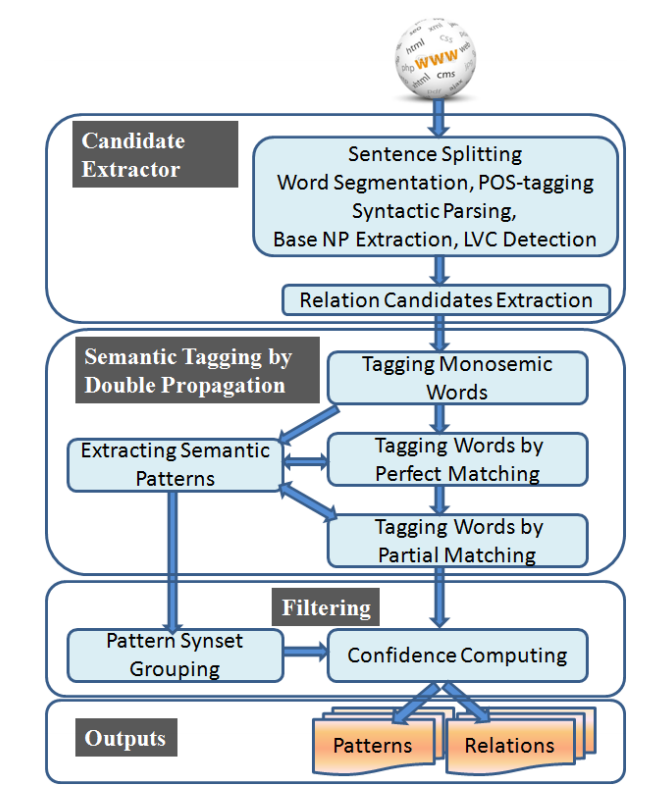
\includegraphics[width=10cm]{ZORE}
\caption{ZORE 体系结构}\label{fig:ZORE}
\end{figure}

\section{ZORE 的简介}
ZORE 的体系结构如图 ~\ref{fig:ZORE} 所示。它由三个部件组成。第一个部件是候选关系提取器,这个提取器获取输入的文本然后进行句子的分割、字词的分割、添加 POS 标签、句法解析、基本的 NP(noun phrase,名词短语) 提取、轻量化的动词结构(LVC,light verb structure)探测和候选关系提取。它的输出是所有候选关系的集合。第二个部件对关系进行添加标签,然后通过双重拓展算法提取语义模式。第三个部件则将被提取出的模式进行同义词集分组,关系则依据“可信分数”进行过滤。

\subsection{提取候选关系}

\subsubsection{解析与基本的 NP 提取}
ZORE 通过应用一系列的 NLP(Natural Language Process,自然语言处理)工具对输入的文本进行流水线处理来分析句法结构。每个句子都通过 Stanford 分割器\citep{chang2008}被分割为一个字词列表,并通过 ZPar \citep{zhang2011}来进行解析,通过标准 CTB \citep{xue2005}来添加 POS 标志和分析结构组成。并对最后生成的构成树使用 Stanford 解析器\citep{chang2008}将其变形为有 Stanford dependencies 的投影树。

接下去,基本的 NPs (名词短语)从依赖树中被提取出来,在这里基本 NP 是一个最大短语,其字词只能拥有来自表 ~\ref{tab:NP} 第一行的 POS。基本 NP 的核心词语可以是一个名词,一个代词,一个数字或是一个量词(表 ~\ref{tab:NP} 的第二行)。基本 NP 里的依赖标签只能来自表 ~\ref{tab:NP} 的第三行。所以,很明显的,一个基本 NP 并不包含其他的基本 NP,并且它本身也不被其他的基本 NP 所包含。

\begin{longtable}{cc}
% 首页表头
\caption[基本 NP 标志表]{包含了 POS 标志和依赖标签,在前三行的标签被用来进行基本 NP 的提取,而最后一行中的标签用于从基本 NP 遍历到谓词短语} \label{tab:NP} \\
\toprule[1.5pt]
  & 标志\\
\midrule[1pt]
\endfirsthead
% 续页表头
\caption[]{(续)} \\
\toprule[1.5pt]
  & 标志\\
\midrule[1pt]
\endhead
% 首页表尾
\hline
\multicolumn{2}{r}{\small 续下页}
\endfoot
% 续页表尾
\bottomrule[1.5pt]
\endlastfoot
基本 NP 修饰语   &   NN (common noun), M (measure word), \\
    &   CD (cardinal number), OD (ordinal number),\\
    &   PN (pronoun), NR(proper noun),\\
    &   NT (temporal noun), \\
    &   JJ (other noun-modifier), or PU (punctuation) \\
    \hline
基本 NP 中的标签  &   nn (noun compound modifier), conj (conjunct),\\
    &   nummod (number modifier),\\
    &   cc (coordinating conjunction),\\
    &   clf (classifier modifier), det (determiner),\\
    &   ordmod (ordinal number modifier),\\
    &   punct (punctuation),\\
    &   dep (other dependencies),\\
    &   or amod (adjectival modifier) \\
    \hline
基本 NP 核心    &   NN (common noun), M (measure word), \\
    &   CD (cardinal number), OD (ordinal number),\\
    &   PN (pronoun), NR(proper noun),\\
    &   NT (temporal noun) \\
    \hline
基本 NP 到谓词的过渡标签  &   nsubj (nominal subject), conj (conjunct),\\
    &   dobj (direct object), advmod (adverbial modifier),\\
    &   prep (preposi-tional modifier),\\
    &   pobj (prepositional object), lobj (localizer object),\\
    &   range (dative object that is a quantifierphrase),\\
    &   tmod (temporal modifier),\\
    &   plmod (localizer modifier of a preposition),\\
    &   attr (attributive), loc (local-izer),\\
    &   top (topic), xsubj (controlling subject),\\
    &   ba (“ba” construction),\\
    &   nsubjpass (nominal passive subject) \\
\end{longtable}

\subsubsection{探测轻量化动词结构}
在语言学中,“轻量化动词”(LVC,light verb construction)指的是一个本身几乎没有语义的动词,并且通常都是和一个名词形成一个谓语\citep{Etzioni2011}。例如,有着“轻量化动词结构”的谓语包括“是国家的”和“宣称拥有主权”,他们的轻量化动词分别是“是”和“宣称”。对 LVC 不合适的处理可能由于不详细的提取导致出现很明显的问题。例如,如果之前两个句子“是国家的”和“宣称拥有主权”中的“是”和“宣称”被作为谓语提取,就会导致提取出的关系无法让人显式地获得有用的信息\citep{Etzioni2011},例如(“税收是国家的收入来源。”,提取出的关系可能是(税收,是,收入来源))。重构动词(ReVerb\citep{Etzioni2011})则解决了以上的问题,通过严格的句法限制让处于动词短语(例如“是”)和介词(例如“的”)中间的名词短语(例如“国家”)被认为是谓词短语的一部分而不是一个参数,从而得出了(税收,是国家的,收入来源)这个关系。

在中文语境中,LVCs 出现的频率非常高,并且应该被妥善地处理,从而保证被提取出的关系可以提供有用的信息。在中文语境中,介词扮演着动词的修饰语,并且可以在动词的左边或右边。例如图 ~\ref{fig:sentence1} 中的例句“侯建国校长就职于中国科学技术大学。”可以被改写为“侯建国校长于中国科学技术大学就职。”,而这两个句子中的介词“于”则分别位于谓词短语“就职”的右边和左边。

中文的 LVCs 可以被归为两类,即“伪 LVC”和“平凡 LVC”。对于伪 LVC,谓词是一个“假的动词”,例如“进行”和“给予”,都是有着名词短语作为他们的对象。因为中文的“假的动词”是一个闭集,我们通过寻找来自语料库的“假的动词”进行探测这种伪 LVC。而对于平凡 LVC,它的谓词则是平凡的动词,即它的谓词有着正常的结构或一个平凡的名词作为对象。例如,“展开调查”就是这种平凡 LVC。


\begin{longtable}{cc}
% 首页表头
\caption[伪 LVC 与平凡 LVC 样例表]{伪 LVC(*) 与平凡 LVC (**)样例表,左列的动词和右列的名词组合生成 LVC,并作为谓词短语。} \label{tab:LVC} \\
\toprule[1.5pt]
动词 & 名词\\
\midrule[1pt]
\endfirsthead
% 续页表头
\caption[]{(续)} \\
\toprule[1.5pt]
动词 & 名词\\
\midrule[1pt]
\endhead
% 首页表尾
\hline
\multicolumn{2}{r}{\small 续下页}
\endfoot
% 续页表尾
\bottomrule[1.5pt]
\endlastfoot
进行(*)   &   发行,分析,收集,修改,访问,处罚\\
    \hline
有(*)  &   影响,贡献,兴趣,帮助,认识,期望\\
    \hline
产生(**)    &   影响,兴趣,怀疑,冲击,好感,恐惧\\
    \hline
造成(**)  &   影响,破坏,伤害,威胁,压力,干扰\\
    \hline
表示(**)  &   满意,欢迎,尊重,担忧,哀悼,感谢\\
    \hline
展开(**)  &   调查,攻击,攻势,批评,批判,诉讼\\
\end{longtable}

平凡 LVC 比伪 LVC 更加难以探测,我们通过上下文的语境来对平凡 LVC 进行探测。包括在 LVC 里的 NP 本身,一个平凡 LVC 通常控制着两个 NP,而处在后面的 NP 则通过一个与 LVC 有关的介词来联系在一起,例如“对,对于,针对,向,同,与,和”。基于以上的现象,一个通用的方法来鉴别平凡 LVC 产生了,即通过寻找在大型语料库中频繁地与 LVC 相关的介词一起出现,被自动解析的动词对象结构。对于一个给定的动词对象 v,用 $f^v$ 和 $f^p$ 分别表示 v 出现的频率和与 v 一起出现的与 LVC 有关的介词的频率。定义 v 成为 LVC 的统计强度为 $f^p / f^v$。如果 v 的统计强度达到了 $t^{lvc}$ 的阈值,则将 v 定义为 LVC。表 ~\ref{tab:LVC} 描述了一些高频率出现的 LVC,通过这种方式被自动提取出来。

\subsubsection{提取候选关系}
ZORE 尝试从含有两个或更多基本 NP 的句子里抽取候选关系。对于给定的两个基本 NP,我们遍历依赖树来获取连结他们的最短路径。而这个最短路径可以仅仅包括表 ~\ref{tab:NP} 中第四行的依赖标志,并且必须包括至少一个来自“nsubj”和“dobj”的标志,从而保证这个谓词短语被包括在最短路径中。如果获取到了这样的最短路径,则其他的被同一个谓词短语所控制的基本 NP 也被包括进了这个目标关系里,得出一个 n 元的候选关系,当中的每个基本 NP 都对应着一个参数。依据这个谓词短语,候选关系可以被归为以下几类:

\newtheorem*{CDLR}{平凡与伪 LVC 关系}
\begin{CDLR}
    在这种关系里,最短路径的谓词短语是一个 LVC(例如一个轻量动词和一个普通的对象)。那两个基本的 NP 可以是轻量动词的前置词或子词。以“老李对我的学业有很大帮助”作为例句,“有”和“帮助”结合形成了一个平凡 LVC,并被当成了一个谓词短语,从而得出了关系(老李,Pred[有帮助],我的学业)。
\end{CDLR}
\newtheorem*{VR}{动词关系}
\begin{VR}
    在这种关系里,一个动词则作为一个谓词短语。例如,这个关系(侯建国校长,Pred[就职],中国科学技术大学)提取自图 ~ref{fig:sentence1} 则是一个典型的动词关系。
\end{VR}
\newtheorem*{RCR}{关联从句关系}
\begin{RCR}
    在这种关系里,核心词语是一个名词,被一个关联从句所修饰,并在语义上作为这个关联从句的谓词的参数。“就职于中国科学技术大学的侯建国校长。”这个句子是图 ~\ref{fig:sentence1} 的一个同义句,有着一样的谓词短语和参数。然而,从这个句子里提取出的关系是一个关联从句关系(Pred[就职],中国科学技术大学,侯建国校长),和图 ~\ref{fig:sentence1} 句子的关系属于一样的模式同义词集。
\end{RCR}

\subsection{双重拓展的语义标注}
基本思想是通过进行对候选关系的参数的核心词语进行词语义标注,迭代地识别关系和模式。对于给定的候选关系集合和语义分类系统,进行拓展包括三个步骤。第一步,候选关系中的单义参数会被用语义类别标注,例如 Af 和 Di,从而获取语义模式。在第二步和第三部,未被标注的的含义模糊和未知词将会分别通过完全匹配和部分匹配进行标注。在每一步的末尾,语义模式来自被提取出和被标注过的关系的概括,之后语义模式被用来帮助下一步的关系标注。因为这种双向的信息交换,这种方式被称之为“双重拓展”。

\subsubsection{第一步:标注单义的参数}
每个在候选关系内的参数都是基本 NP,因为基本 NP 都是向心结构的\citep{endocentric2017},所以我们可以将一个基本 NP 的核心词语语义类别当作这个基本 NP 的语义类别。在一个分类系统里,每个字词都和一个或更多的语义类别有关。然而,在这步里,只有单义的词语才会被标注,而词义模糊和未知的词语都会被忽略,不会被标注。

大部分被命名的实体并没有被包括在分类系统中。然而,在标注了 POS 标签后,大部分的已命名实体将会被探测为 NR(proper noun,专有名词)。而这导致那些已命名的实体将会被作为词义模糊的词语处理,可以是人名,组织名,或地名。未被分类系统包括的已命名实体将会在第二、三步里被标注。

在这步之后,在一些候选关系里的所有参数都已经被用语义分类标注。这些候选关系被称为“已标注候选关系”,而其他的候选关系则被称之为“未标注候选关系”。已标注候选关系将会被归纳为语义模式,包括句法模式和语义标签,就像图 ~\ref{fig:sentence1} 里所描述的。将由此生成的语义模式称之为$Set^{SemPat}$

\subsubsection{第二步:完全的模式匹配标注}
在这步,将会通过语义模式匹配对未标注候选关系里的参数进行标注。对于给定的未标注候选关系 r,我们对每一个有着模糊词义的核心词语,获取一个潜在语义类型集合。对于有着未知核心词语的参数,我们根据他们的单字获取潜在语义类型集合。98\% 的中文字词至少都有一个同义字词\citep{qiu2011},并且原字词和同义字词之间至少有一个字一样。对于中文名词,同义字词的集合通常也有着至少一或二个一样的字。所以,对于获取未知字词的潜在的词义类型策略就大致成型了。

首先,对于给定的未知字词 $w^u$,如果我们可以发现一个已知的字词 $w^k$ 与未知的字词 $w^u$ 结尾的两个字一样,则 $w^k$ 的语义类型会被作为 $w^u$ 的潜在语义类型。否则,如果 $w^u$ 和 $w^k$ 最后一个字都一样,那么 $w^k$ 的语义类型会被作为 $w^u$ 的潜在语义类型。

接下去我们开始获取未标注的候选关系的潜在语义标签,这里的未标注候选关系的所有参数已经被潜在语义类型所标注。就像第一步里的,我们将关系 $r$ 归纳为一个句法模式 $pat^{syn}$,之后将 $pat^{syn}$ 与每一个 $r$ 的潜在语义标签来生成潜在语义模式。为了避免一个或更多 $r$ 的潜在语义模式存在于 $Set^{SemPat}$ 中,如果那些语义模式当中频率最高的模式超过了阈值 $t^{sem}$ ,那么符合条件的模式将会被作为 $r$ 的语义模式,由此我们推断 $r$ 的语义标志和之后 $r$ 的每个参数的核心词语的语义类型。做完这步以后,每个语义模式在 $Set^{SemPat}$ 中的频率都会依据最新被标注的候选关系进行更新。

\subsubsection{第三步:部分的模式匹配标注}
在这步,我们标注含混的和未知的字词,通过部分的匹配而不是完全的整个语义模式的匹配。这被当作一个最后一步的补偿。

我们首先将 $Set^{SemPat}$ 中的一个 n 元语义模式分割为二元语义模式,并计算它们的频率。之后,我们将每个未标注的候选关系 $r$ 分割为几个二元的子关系,并从每一个二元的子关系搜索符合与第二步一样的条件的语义模式。对于每个二元的子关系,我们获取最高频率的二元语义标志。之后通过结合二元语义标志,我们就可以获取 $r$ 的一个 n 元的语义标签,基于这个语义标签,所有的未知和含混的字词都可以被语义类型所标注。如果一个候选关系 $r$ 的所有的参数已经被标注,那么 $r$ 可以被当作已经被标注。最后,根据最新的被标注的关系,$Set^{SemPat}$ 中的统计数据也将被更新。

\subsection{将模式分组为同义词集}
在这步,我们将来自 $Set^{SemPat}$ 中的语义模式分组为模式同义词集,基于一个单通道的聚类过程\citep{papka1998}。对于给定的两个语义模式 $SemPat_i$ 和 $SemPat_j$,我们分别以 $SynPat_i$,$SynPat_j$,$SemSIg_i$,$SenSig_i$,$Pred_i$,$Pred_i$ 来表示他们所导出的句法模式、语义标志、谓词短语。在忽略谓词短语的情况下,$SynPat_i$  和 $SynPat_j$ 是完全相同的,并且在这种前提下我们称他们的关系为为约等于($ \approx$)。

\begin{algorithm}[htbp]
\SetAlgoLined
\SetKw{KwA}{and}
\SetKw{KwO}{or}
    \uIf{$Pred_i$ = “是” \KwO $Pred_j$ = “是”}{
        \KwRet{$false$}\;
    }
    \uElseIf{$ArgCount(SemPat_i) = 2$ \KwA $ArgCount(SemPat_j) = 2$ \KwA $SemCat(arg_1) = SemCat(arg_2)$}{
        \uIf{$SynPat_i \approx SynPat_j$ \KwA $IsSynonym(Pred_i, Pred_j$)}{
            \KwRet{$true$}\;
        }
        \uElseIf{$Pred_i = Pred_j$}{
            \KwRet{$true$}\;
        }
        \Else{
            \KwRet{$false$}\;
        }
    }
    \uElseIf{$Pred_i = Pred_j$ \KwA $SemSig_i = SemSig_j$}{
        \KwRet{$true$}\;
    }
    \uElseIf{$IsSynonym(Pred_i, Pred_j)$ \KwA $SemSig_i = SemSig_j$ \KwA $SynPat_i \approx SynPat_j$}{
        \KwRet{$true$}\;
    }
    \Else{
        \KwRet{$false$}\;
    }
\caption[模式同义词集分组]{模式同义词集分组}
\label{algo:grouping}
\end{algorithm}

算法 \ref{algo:grouping} 的功能为对模式进行分组,其中 $ArgCount(SynPat_i)$ 表示在 $SynPat_i$ 中的参数的数量,$SemCat(Arg_1)$ 则表示第一个参数的语义类别,$IsSynonym(Pred_i, Pred_j)$ 则会得出入参的这两个谓词是否是同义词。在基于相似性的单通道聚类中,主题偏移的问题十分常见\citep{papka1998}。但是因为这里的相似性测度是均匀的,所以算法 \ref{algo:grouping} 并不会受到主题偏移的影响。

\subsection{计算关系的置信度}
在没有过滤的情况下,
\chapter{中文开放式关系抽取}
\label{chap:zore}

中文开放式关系抽取(ZORE)\citep{ZORE} 的体系结构如图 ~\ref{fig:ZORE} 所示。它由三个部件组成。第一个部件是候选关系提取器,这个提取器获取输入的文本然后进行句子的分割、字词的分割、添加 POS 标签、句法解析、基本的 NP(noun phrase,名词短语) 提取、轻量化的动词结构(LVC,light verb structure)探测和候选关系提取。它的输出是所有候选关系的集合。第二个部件对关系进行添加标签,然后通过双重拓展算法提取语义模式。第三个部件则将被提取出的模式进行同义词集分组,关系则依据“可信分数”进行过滤。
先前的对于英文语境下的 ORE 研究从浅句法发展至全句法,然后是语义系统。这显示了一个基于语法依存的全句法分析的系统相对于基于表面的“POS 模式”的浅句法分析系统可以得出显著更加优越的分析结果,然而语义系统却比前二者拥有更高效率且更精准的分析结果。

\begin{figure}[h]
\centering
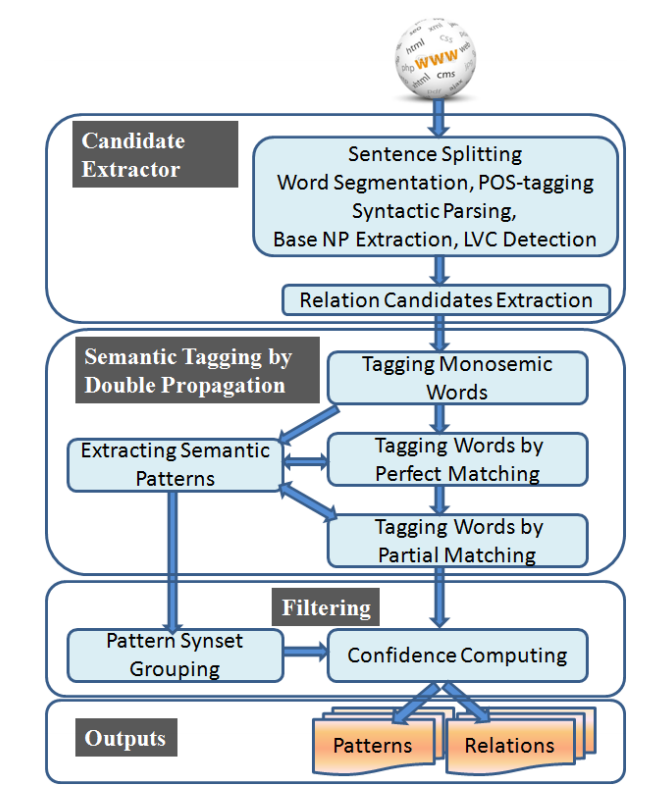
\includegraphics[width=10cm]{ZORE}
\caption{ZORE 体系结构}\label{fig:ZORE}
\end{figure}

\begin{figure}[h]
\centering
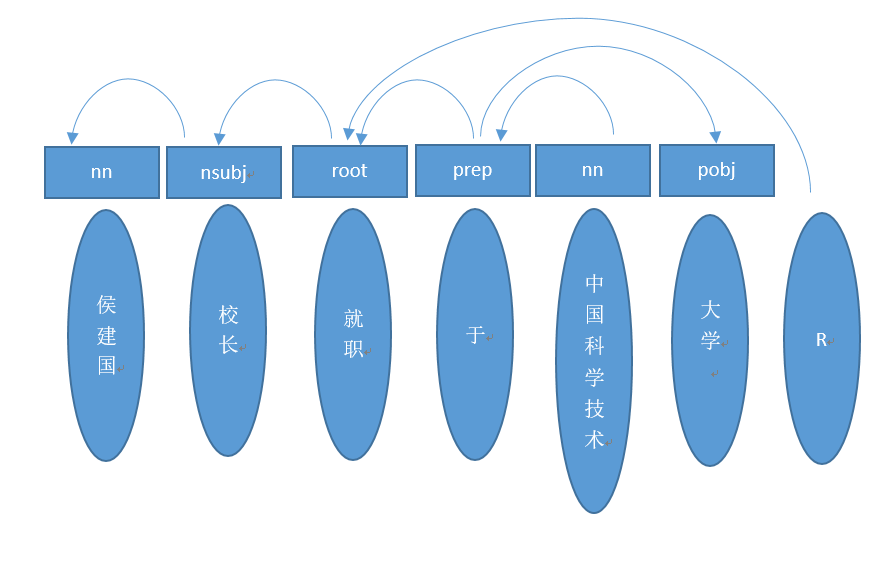
\includegraphics[width=12cm]{parseSentence}
\caption[句子解析结果]{以 StanFord 依存关系对例句“侯建国校长就职于中国科学技术大学”进行解析的结果}\label{fig:parseSentence}
\end{figure}

本文使用的中文语境下的 ORE 系统基于全依存句法分析,并且可以识别涉及长距离依存的模式。鉴于中文的特点,例如缺少功能词\citep{funcword}与形态学\citep{morphword},并且有着较高的词义模糊性与分段性,ZORE 我们将语义本体信息结合到系统的设计中,以提高输出质量,而不会降低效率。

当前使用最新技术的系统是 PAYYT\citep{naka2012},也是基于全依存句法分析,但其为英文语境下的关系抽取系统。并且他们是首先抽取关系再基于抽取的关系对模式进行精细化。ZORE 则将抽取关系与精细化模式同步进行,从而可以让二者互相提升。先前的研究显示模式归纳受益于关系提取\citep{naka2012},并且关系提取也可以受益于模式归纳\citep{mau2012}。通过使用双重拓展算法,不仅可以让模式与关系的提取相互受益,还可以在同一个过程里进行对模式与关系语义类型的标注。

对于中文语境下的关系抽取也有其他的方式,例如基于特征的方法与基于内核的方法。然而,其他的中文语境下的关系抽取都是关注于有着预先定义的关系的传统的信息抽取。语义本体亦是中文语境下的关系抽取里有用的一个定义,却基本没有被使用。并且,那些系统可以被视为一个流水线,依次进行分词、POS 标签标注、解析。ZORE 则给出了语义解释,并通过一种新颖的双重拓展算法在模式和关系之间明确地处理解析中的统计误差。

\section{提取候选关系}

\subsection{解析与基本的 NP 提取}
ZORE 通过应用一系列的 NLP(Natural Language Process,自然语言处理)工具对输入的文本进行流水线处理来分析句法结构。每个句子都通过 Stanford 分割器\citep{chang2008}被分割为一个字词列表,并通过 ZPar \citep{zhang2011}来进行解析,通过标准 CTB \citep{xue2005}来添加 POS 标志和分析结构组成。并对最后生成的构成树使用 Stanford 解析器\citep{chang2008}将其变形为有 Stanford dependencies 的投影树。

接下去,基本的 NPs (名词短语)从依存树中被提取出来,在这里基本 NP 是一个最大短语,其字词只能拥有来自表 ~\ref{tab:NP} 第一行的 POS。

\begin{longtable}{cc}
% 首页表头
\caption[基本 NP 标志表]{包含了 POS 标志和依存标签,在前三行的标签被用来进行基本 NP 的提取,而最后一行中的标签用于从基本 NP 遍历到谓词短语} \label{tab:NP} \\
\toprule[1.5pt]
  & 标志\\
\midrule[1pt]
\endfirsthead
% 续页表头
\caption[]{基本 NP 标志表(续)} \\
\toprule[1.5pt]
  & 标志\\
\midrule[1pt]
\endhead
% 首页表尾
\hline
\multicolumn{2}{r}{\small 续下页}
\endfoot
% 续页表尾
\bottomrule[1.5pt]
\endlastfoot
基本 NP 修饰语   &   NN (common noun), M (measure word), \\
    &   CD (cardinal number), OD (ordinal number),\\
    &   PN (pronoun), NR(proper noun),\\
    &   NT (temporal noun), \\
    &   JJ (other noun-modifier), or PU (punctuation) \\
    \hline
基本 NP 中的标签  &   nn (noun compound modifier), conj (conjunct),\\
    &   nummod (number modifier),\\
    &   cc (coordinating conjunction),\\
    &   clf (classifier modifier), det (determiner),\\
    &   ordmod (ordinal number modifier),\\
    &   punct (punctuation),\\
    &   dep (other dependencies),\\
    &   or amod (adjectival modifier) \\
基本 NP 核心    &   NN (common noun), M (measure word), \\
    &   CD (cardinal number), OD (ordinal number),\\
    &   PN (pronoun), NR(proper noun),\\
    &   NT (temporal noun) \\
    \hline
基本 NP 到谓词的过渡标签  &   nsubj (nominal subject), conj (conjunct),\\
    &   dobj (direct object), advmod (adverbial modifier),\\
    &   prep (preposi-tional modifier),\\
    &   pobj (prepositional object), lobj (localizer object),\\
    &   range (dative object that is a quantifierphrase),\\
    &   tmod (temporal modifier),\\
    &   plmod (localizer modifier of a preposition),\\
    &   attr (attributive), loc (local-izer),\\
    &   top (topic), xsubj (controlling subject),\\
    &   ba (“ba” construction),\\
    &   nsubjpass (nominal passive subject) \\
\end{longtable}

基本 NP 的核心词语可以是一个名词,一个代词,一个数字或是一个量词(表 ~\ref{tab:NP} 的第二行)。基本 NP 里的依存标签只能来自表 ~\ref{tab:NP} 的第三行。所以,很明显的,一个基本 NP 并不包含其他的基本 NP,并且它本身也不被其他的基本 NP 所包含。

\subsection{探测轻量化动词结构}
在语言学中,“轻量化动词”(LVC,light verb construction)指的是一个本身几乎没有语义的动词,并且通常都是和一个名词形成一个谓语\citep{Etzioni2011}。例如,有着“轻量化动词结构”的谓语包括“是国家的”和“宣称拥有主权”,他们的轻量化动词分别是“是”和“宣称”。对 LVC 不合适的处理可能由于不详细的提取导致出现很明显的问题。例如,如果之前两个句子“是国家的”和“宣称拥有主权”中的“是”和“宣称”被作为谓语提取,就会导致提取出的关系无法让人显式地获得有用的信息\citep{Etzioni2011},例如(“税收是国家的收入来源。”,提取出的关系可能是(税收,是,收入来源))。重构动词(ReVerb\citep{Etzioni2011})则解决了以上的问题,通过严格的句法限制让处于动词短语(例如“是”)和介词(例如“的”)中间的名词短语(例如“国家”)被认为是谓词短语的一部分而不是一个论元,从而得出了(税收,是国家的,收入来源)这个关系。

在中文语境中,LVCs 出现的频率非常高,并且应该被妥善地处理,从而保证被提取出的关系可以提供有用的信息。在中文语境中,介词扮演着动词的修饰语,并且可以在动词的左边或右边。例如图 ~\ref{fig:sentence1} 中的例句“侯建国校长就职于中国科学技术大学。”可以被改写为“侯建国校长于中国科学技术大学就职。”,而这两个句子中的介词“于”则分别位于谓词短语“就职”的右边和左边。

中文的 LVCs 可以被归为两类,即“伪 LVC”和“平凡 LVC”。对于伪 LVC,谓词是一个“假的动词”,例如“进行”和“给予”,都是有着名词短语作为他们的对象。因为中文的“假的动词”是一个闭集,我们通过寻找来自语料库的“假的动词”进行探测这种伪 LVC。而对于平凡 LVC,它的谓词则是平凡的动词,即它的谓词有着正常的结构或一个平凡的名词作为对象。例如,“展开调查”就是这种平凡 LVC。

\begin{longtable}{cc}
% 首页表头
\caption[伪 LVC 与平凡 LVC 样例表]{伪 LVC(*) 与平凡 LVC (**)样例表,左列的动词和右列的名词组合生成 LVC,并作为谓词短语。} \label{tab:LVC} \\
\toprule[1.5pt]
动词 & 名词\\
\midrule[1pt]
\endfirsthead
% 续页表头
\caption[]{伪 LVC(*) 与平凡 LVC (**)样例表(续)} \\
\toprule[1.5pt]
动词 & 名词\\
\midrule[1pt]
\endhead
% 首页表尾
\hline
\multicolumn{2}{r}{\small 续下页}
\endfoot
% 续页表尾
\bottomrule[1.5pt]
\endlastfoot
进行(*)   &   发行,分析,收集,修改,访问,处罚\\
    \hline
有(*)  &   影响,贡献,兴趣,帮助,认识,期望\\
    \hline
产生(**)    &   影响,兴趣,怀疑,冲击,好感,恐惧\\
    \hline
造成(**)  &   影响,破坏,伤害,威胁,压力,干扰\\
    \hline
表示(**)  &   满意,欢迎,尊重,担忧,哀悼,感谢\\
    \hline
展开(**)  &   调查,攻击,攻势,批评,批判,诉讼\\
\end{longtable}

平凡 LVC 比伪 LVC 更加难以探测,我们通过上下文的语境来对平凡 LVC 进行探测。包括在 LVC 里的 NP 本身,一个平凡 LVC 通常控制着两个 NP,而处在后面的 NP 则通过一个与 LVC 有关的介词来联系在一起,例如“对,对于,针对,向,同,与,和”。基于以上的现象,一个通用的方法来鉴别平凡 LVC 产生了,即通过寻找在大型语料库中频繁地与 LVC 相关的介词一起出现,被自动解析的动词对象结构。对于一个给定的动词对象 v,用 $f^v$ 和 $f^p$ 分别表示 v 出现的频率和与 v 一起出现的与 LVC 有关的介词的频率。定义 v 成为 LVC 的统计强度为 $f^p / f^v$。如果 v 的统计强度达到了 $t^{lvc}$ 的阈值,则将 v 定义为 LVC。表 ~\ref{tab:LVC} 描述了一些高频率出现的 LVC,通过这种方式被自动提取出来。

\subsection{提取候选关系}
ZORE 尝试从含有两个或更多基本 NP 的句子里抽取候选关系。对于给定的两个基本 NP,我们遍历依存树来获取连结他们的最短路径。而这个最短路径可以仅仅包括表 ~\ref{tab:NP} 中第四行的依存标志,并且必须包括至少一个来自“nsubj”和“dobj”的标志,从而保证这个谓词短语被包括在最短路径中。如果获取到了这样的最短路径,则其他的被同一个谓词短语所控制的基本 NP 也被包括进了这个目标关系里,得出一个 n 元的候选关系,当中的每个基本 NP 都对应着一个论元。依据这个谓词短语,候选关系可以被归为以下几类:

\newtheorem*{CDLR}{平凡与伪 LVC 关系}
\begin{CDLR}
    在这种关系里,最短路径的谓词短语是一个 LVC(例如一个轻量动词和一个普通的对象)。那两个基本的 NP 可以是轻量动词的前置词或子词。以“老李对我的学业有很大帮助”作为例句,“有”和“帮助”结合形成了一个平凡 LVC,并被当成了一个谓词短语,从而得出了关系(老李,Pred[有帮助],我的学业)。
\end{CDLR}
\newtheorem*{VR}{动词关系}
\begin{VR}
    在这种关系里,一个动词则作为一个谓词短语。例如,这个关系(侯建国校长,Pred[就职],中国科学技术大学)提取自图 ~ref{fig:sentence1} 则是一个典型的动词关系。
\end{VR}
\newtheorem*{RCR}{关联从句关系}
\begin{RCR}
    在这种关系里,核心词语是一个名词,被一个关联从句所修饰,并在语义上作为这个关联从句的谓词的论元。“就职于中国科学技术大学的侯建国校长。”这个句子是图 ~\ref{fig:sentence1} 的一个同义句,有着一样的谓词短语和论元。然而,从这个句子里提取出的关系是一个关联从句关系(Pred[就职],中国科学技术大学,侯建国校长),和图 ~\ref{fig:sentence1} 句子的关系属于一样的模式同义词集。
\end{RCR}

\section{双重拓展的语义标注}
基本思想是通过进行对候选关系的论元的核心词语进行词语义标注,迭代地识别关系和模式。对于给定的候选关系集合和语义分类系统,进行拓展包括三个步骤。第一步,候选关系中的单义论元会被用语义类别标注,例如 Af 和 Di,从而获取语义模式。在第二步和第三部,未被标注的的含义模糊和未知词将会分别通过完全匹配和部分匹配进行标注。在每一步的末尾,语义模式来自被提取出和被标注过的关系的概括,之后语义模式被用来帮助下一步的关系标注。因为这种双向的信息交换,这种方式被称之为“双重拓展”。

\subsection{第一步:标注单义的论元}
每个在候选关系内的论元都是基本 NP,因为基本 NP 都是向心结构的\citep{endocentric2017},所以我们可以将一个基本 NP 的核心词语语义类别当作这个基本 NP 的语义类别。在一个分类系统里,每个字词都和一个或更多的语义类别有关。然而,在这步里,只有单义的词语才会被标注,而词义模糊和未知的词语都会被忽略,不会被标注。

大部分被命名的实体并没有被包括在分类系统中。然而,在标注了 POS 标签后,大部分的已命名实体将会被探测为 NR(proper noun,专有名词)。而这导致那些已命名的实体将会被作为词义模糊的词语处理,可以是人名,组织名,或地名。未被分类系统包括的已命名实体将会在第二、三步里被标注。

在这步之后,在一些候选关系里的所有论元都已经被用语义分类标注。这些候选关系被称为“已标注候选关系”,而其他的候选关系则被称之为“未标注候选关系”。已标注候选关系将会被归纳为语义模式,包括句法模式和语义标签,就像图 ~\ref{fig:sentence1} 里所描述的。将由此生成的语义模式称之为$Set^{SemPat}$

\subsection{第二步:完全的模式匹配标注}
在这步,将会通过语义模式匹配对未标注候选关系里的论元进行标注。对于给定的未标注候选关系 r,我们对每一个有着模糊词义的核心词语,获取一个潜在语义类型集合。对于有着未知核心词语的论元,我们根据他们的单字获取潜在语义类型集合。98\% 的中文字词至少都有一个同义字词\citep{qiu2011},并且原字词和同义字词之间至少有一个字一样。对于中文名词,同义字词的集合通常也有着至少一或二个一样的字。所以,对于获取未知字词的潜在的词义类型策略就大致成型了。

首先,对于给定的未知字词 $w^u$,如果我们可以发现一个已知的字词 $w^k$ 与未知的字词 $w^u$ 结尾的两个字一样,则 $w^k$ 的语义类型会被作为 $w^u$ 的潜在语义类型。否则,如果 $w^u$ 和 $w^k$ 最后一个字都一样,那么 $w^k$ 的语义类型会被作为 $w^u$ 的潜在语义类型。

接下去我们开始获取未标注的候选关系的潜在语义标签,这里的未标注候选关系的所有论元已经被潜在语义类型所标注。就像第一步里的,我们将关系 $r$ 归纳为一个句法模式 $pat^{syn}$,之后将 $pat^{syn}$ 与每一个 $r$ 的潜在语义标签来生成潜在语义模式。为了避免一个或更多 $r$ 的潜在语义模式存在于 $Set^{SemPat}$ 中,如果那些语义模式当中频率最高的模式超过了阈值 $t^{sem}$ ,那么符合条件的模式将会被作为 $r$ 的语义模式,由此我们推断 $r$ 的语义标志和之后 $r$ 的每个论元的核心词语的语义类型。做完这步以后,每个语义模式在 $Set^{SemPat}$ 中的频率都会依据最新被标注的候选关系进行更新。

\subsection{第三步:部分的模式匹配标注}
在这步,我们标注含混的和未知的字词,通过部分的匹配而不是完全的整个语义模式的匹配。这被当作一个最后一步的补偿。

我们首先将 $Set^{SemPat}$ 中的一个 n 元语义模式分割为二元语义模式,并计算它们的频率。之后,我们将每个未标注的候选关系 $r$ 分割为几个二元的子关系,并从每一个二元的子关系搜索符合与第二步一样的条件的语义模式。

对于每个二元的子关系,我们获取最高频率的二元语义标志。之后通过结合二元语义标志,我们就可以获取 $r$ 的一个 n 元的语义标签,基于这个语义标签,所有的未知和含混的字词都可以被语义类型所标注。如果一个候选关系 $r$ 的所有的论元已经被标注,那么 $r$ 可以被当作已经被标注。最后,根据最新的被标注的关系,$Set^{SemPat}$ 中的统计数据也将被更新。

\section{将模式分组为同义词集}

\begin{algorithm}[!h]
\SetAlgoLined
\SetKw{KwA}{and}
\SetKw{KwO}{or}
    \uIf{$Pred_i$ = “是” \KwO $Pred_j$ = “是”}{
        \KwRet{$false$}\;
    }
    \uElseIf{$ArgCount(SemPat_i) = 2$ \KwA $ArgCount(SemPat_j) = 2$ \KwA $SemCat(arg_1) = SemCat(arg_2)$}{
        \uIf{$SynPat_i \approx SynPat_j$ \KwA $IsSynonym(Pred_i, Pred_j$) \KwO $Pred_i = Pred_j$}{
            \KwRet{$true$}\;
        }
        \Else{
            \KwRet{$false$}\;
        }
    }
    \uElseIf{$Pred_i = Pred_j$ \KwA $SemSig_i = SemSig_j$ \KwO $IsSynonym(Pred_i, Pred_j)$ \KwA $SemSig_i = SemSig_j$ \KwA $SynPat_i \approx SynPat_j$}{
        \KwRet{$true$}\;
    }
    \Else{
        \KwRet{$false$}\;
    }
\caption[模式同义词集分组]{模式同义词集分组}
\label{algo:grouping}
\end{algorithm}

在这步,我们将来自 $Set^{SemPat}$ 中的语义模式分组为模式同义词集,基于一个单通道的聚类过程\citep{papka1998}。

对于给定的两个语义模式 $SemPat_i$ 和 $SemPat_j$,我们分别以 $SynPat_i$,$SynPat_j$,$SemSIg_i$,$SenSig_i$,$Pred_i$,$Pred_i$ 来表示他们所导出的句法模式、语义标志、谓词短语。在忽略谓词短语的情况下,$SynPat_i$  和 $SynPat_j$ 是完全相同的,并且在这种前提下我们称他们的关系为为约等于($ \approx$)。

算法 \ref{algo:grouping} 的功能为对模式进行分组,其中 $ArgCount(SynPat_i)$ 表示在 $SynPat_i$ 中的论元的数量,$SemCat(Arg_i)$ 表示第 i 个论元的语义类别,而以两个谓词入参的 $IsSynonym(Pred_i, Pred_j)$ 则会得出入参的这两个谓词是否是同义词。

在基于相似性的单通道聚类中,主题偏移的问题十分常见\citep{papka1998}。但是因为这里的相似性测度是均匀的,所以算法 \ref{algo:grouping} 并不会受到主题偏移的影响。

\section{计算关系的置信度}
在没有过滤的情况下,算法 \ref{algo:grouping} 的提取可能产出不正确的关系。根据以前的 ORE 系统,我们可以使用一个置信度的阈值来达到召回与精确之间的平衡。

一种Logistic 回归分类器被用来为每一个关系进行置信度分数的计算,他们的特征值在表 ~\ref{tab:feature} 中展示。在这个表中,$c$,$r$,$arguments$,$SemPat$ 分别表示从句(Clause),关系(Relation),关系中的论元,语义模式(Semantic Pattern)。$Length(r)$,$Count(arguments)$,$Size(SemPat)$ 分别表示 $r$ 中的字数,$r$ 中的论元个数,和 $r$ 的语义模式 $SemPat$ 一样的关系的数量。因为从双重拓展中提取出的语义模式被用作分类器中的特征,所以他们也参与了关系抽取。他们对关系抽取的影响可以直接体现在双重拓展算法的效率中。

\begin{longtable}{ccc}
% 首页表头
\caption[Logistic 回归分类器特征表]{带权重的Logistic 回归分类器特征,通过 Wiki-500 的数据进行训练所得出。} \label{tab:feature} \\
\toprule[1.5pt]
类型 & 特征 & 权重\\
\midrule[1pt]
\endfirsthead
% 续页表头
\caption[]{Logistic 回归分类器特征表(续)} \\
\toprule[1.5pt]
类型 & 特征 & 权重\\
\midrule[1pt]
\endhead
% 首页表尾
\hline
\multicolumn{3}{r}{\small 续下页}
\endfoot
% 续页表尾
\bottomrule[1.5pt]
\endlastfoot
基本(Base)   &   $r$ 覆盖了 $c$ 中所有词语           &   0.96\\
基本(Base)   &   $r$ 中有逗号                        &   -0.47\\
基本(Base)   &   $Length(r) < 10 个字$              &   0.35\\
基本(Base)   &   $10 个字 \leq Length(r) < 20个字$ &   0.11\\
基本(Base)   &   $Length(r) < 20个字$             &   -1.06\\
基本(Base)   &   $Count(arguments) = 2$             &   0.14\\
基本(Base)   &   $Count(arguments) = 3$             &   0.33\\
基本(Base)   &   $Count(arguments) = 4$             &   -0.60\\
基本(Base)   &   $Count(arguments) > 4$           &   -0.46\\
    \hline
词义模式(SemPat)  &   在第三步中被标注                 &  0.87\\
词义模式(SemPat)  &   在第三步前被标注                 &  0.75\\
词义模式(SemPat)  &   $50 \leq Size(SemPat)$且未被标注 &  -0.05\\
词义模式(SemPat)  &   $50 \leq Size(SemPat)$且已被标注 &  0.65\\
词义模式(SemPat)  &   $10 \leq Size(SemPat) < 50$且未被标注 &  -0.16\\
词义模式(SemPat)  &   $10 \leq Size(SemPat) < 50$且已被标注 &  0.39\\
词义模式(SemPat)  &   $5 \leq Size(SemPat) < 10$且未被标注 &  -0.22\\
词义模式(SemPat)  &   $5 \leq Size(SemPat) < 10$且已被标注 &  0.36\\
词义模式(SemPat)  &   $Size(SemPat) < 5$且未被标注 &  -0.92\\
词义模式(SemPat)  &   $Size(SemPat) < 5$且已被标注 &  -0.64\\
\end{longtable}

\section{本章小结}
这一章的内容集中介绍了 ZORE 系统的架构与其对中文文本的关系抽取过程,包括分词、词性标注、依存句法分析、双重拓展算法的介绍和 $Logistic$ 置信度的计算方法,为下一章进行实验做好准备。

\chapter{实验分析}
本文基于第三章里所提及的 ZORE 系统来进行中文文本的关系抽取。当中包括了 ZORE 在试验的语料库上的运行及其抽取关系实验。本章首先介绍了当前主流的对于开放式关系抽取算法评价指标,之后介绍了如何获取对当前算法评估所需的数据以及将 ZORE 算法与 DPM 算法进行对比,列出并分析了实验结果以及实验中出现的错误出现原因,提出基于实验数据的对 ZORE 进行性能提高设想。
\section{评判标准}对于 ZORE 系统的评判指标,此处使用主流论文对于开放式关系抽取算法的评价指标:准确率(Precision)、召回率(Recall)、综合评价 F1 值。

为了精确地统计 ZORE 系统运行关系抽取功能于各语料库内的性能数据,采用人工对抽取结果进行检查。实验数据的统计方法为:第一步,对 ZORE 算法的抽取结果进行人工标注,判断其求出的关系元组是否符合人的理解方式,若符合,则将该组标注为 $True$,反之则标注为 $False$,$T$ 为全部的有 $True$ 标记的关系元组集,$N$ 则为全部的有 $False$ 标记的关系元组集,$A$ 表示所有被抽取出的关系元组集,$A=T\cup N$。$S$ 则表示人工对语料库标注的实际正确关系集合。
    \begin{equation}
        Precision=\frac{|T|}{|A|}\times 100\%
    \end{equation}
    \begin{equation}
        Recall=\frac{|T|}{|S|}\times 100\%
    \end{equation}
    \begin{equation}
        F1=\frac{2\times Precision\times Recall}{Precision+Recall}
    \end{equation}

显然,Precision 为算法所求得的正确关系元组数占所有关系元组的百分比,算法抽取的关系的正确结果比例随着 Precision 的升高而升高。召回率则表示算法所求出的正确关系占实际正确关系的比例,可以提供算法抽取关系是否全面的评价指标,随着比例增高遗漏实际正确关系的概率会降低。普遍状态下,召回率与精确率成反比,即召回率越高精确率越低,故还有指标 F1 来评价算法的综合性能,显然,F1 越大则算法全面表现越出色。

\section{实验环境构建}
操作系统:Windows10,java version 1.8.0\_131,IDE 使用 Eclipse。在语料库“燃规3”中运行 ZORE。本语料库经过过滤“燃规3”中未以标点符号结尾的句子后,由 331 个句子构成,而中文词典《同义词林》\citep{che2005}则被用来提供每个字词的语义类别。《同义词林》包含了 77492 个中文字词,并被组织为五级的分层。在顶层有 12 个类别,第二、第三层则分别有 94 和 1492 个类别。在 ZORE 系统中以第二层的类别作为语义分类基准。而模式匹配的阈值 $t^{lvc}$ 与 $t^{sem}$ 分别设置为 0.4 与 3。

对于实验文本的数据集,因为是法规类文本,所以需要对每个条目开头的数字编号进行处理,以避免进行关系抽取时这些数字对关系抽取产生影响。因为每个条目开头数字编号的结构是“数字.数字.数字”,即 python 下的正则表达式类型为 $\backslash d\backslash .\backslash d\backslash .\backslash d$。以下为 python 对文本数据的预处理:

\begin{lstlisting}[language=python, caption=python 文本预处理, label={code:pythonpreprocess}]
import re

fo = open("foo.txt", "r")
bar = open("foo_modified.txt", "w")
while 1:
    line = fo.readline()
    if not line:
        break
    line = re.sub("\d\.\d\.\d", "", line)
    bar.write(line)
fo.close()
bar.close()
\end{lstlisting}

对输入文本进行完去除噪声处理之后,便可以开始使用 ZORE 对文本进行处理。处理完成后,ZORE 将文本中抽取出的关系以 $*.xml$ 的方式进行存储,图 ~\ref{fig:result} 表示了 ZORE 从“燃规3”中的一个句子里提取出的关系。

输出的关系文件当中存在 ZPar 依存分析的标签,各标签的含义如表 ~\ref{tab:ZParDep}。

\begin{longtable}{|c|c|c|c|}
% 首页表头
\caption[ZPar 依存分析标签]{ZPar 依存分析的标签} \label{tab:ZParDep} \\
\toprule[1.5pt]
 标签 & 含义 & 标签 & 含义 \\
\midrule[1pt]
\endfirsthead
% 续页表头
\caption[]{ZPar 依存分析的标签(续)} \\
\toprule[1.5pt]
 标签 & 含义 & 标签 & 含义 \\
\midrule[1pt]
\endhead
% 首页表尾
\hline
\multicolumn{4}{r}{\small 续下页}
\endfoot
% 续页表尾
\bottomrule[1.5pt]
\endlastfoot
    ROOT    &   核心关系    &  VOB     &   动宾关系    \\
    \hline
    RAD     &   右附加关系    & RED    &   重复元素    \\
    \hline
    SBV     &   主谓关系     & RADC    &   非共享右附加关系    \\
    \hline
    PUS     &   句中标点      & IOB    &   间宾关系    \\
    \hline
    POB    &   介词宾语      & ACT    &   动词性宾语    \\
    \hline
    ATT    &   定中关系     & ADV    &   状中关系    \\
    \hline
    CMP    &   动补关系      & APP    &   同位语关系    \\
    \hline
    COO    &   并列关系      & COS    &   右共享并列关系    \\
    \hline
    IC    &   独立子句     & IS    &   独立结构    \\
    \hline
    PUN    &   句末标点      &  TPC    &   主题    \\
    \hline
    VV    &   串行动词      & MT    &   时态    \\
    \hline
    NUM    &   数量      & QUN    &   度量关系    \\
    \hline
    QUC    &   前置量词     & QUCC    &   非共享前置量词    \\
    \hline
     ISC    &   非共享独立结构      & LAD    &   左附加关系    \\
\end{longtable}

因为 ZORE 利用 ZPar 进行依存句法分析,所以输出的关系文件当中存在 ZPar 所定义的词性标注的标签,各标签的含义如表 ~\ref{tab:ZParSem}。

\begin{figure}[htb]
\centering
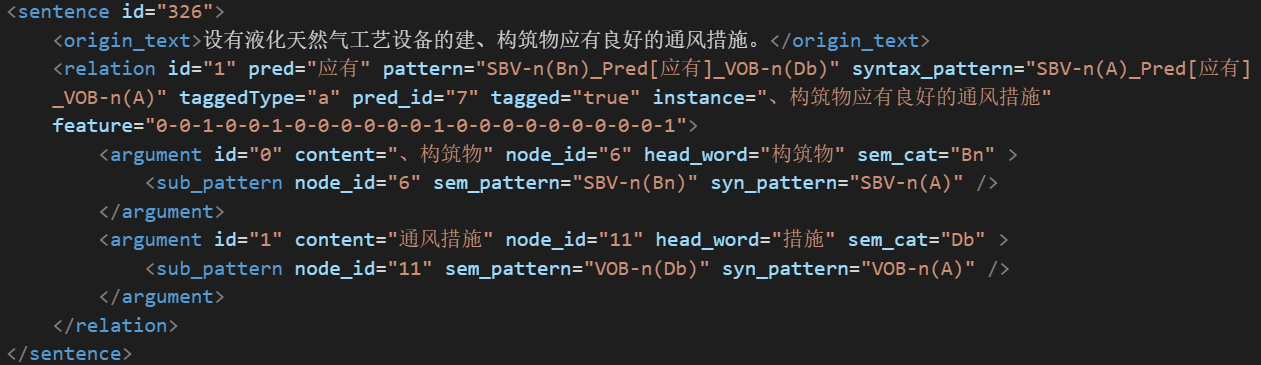
\includegraphics[width=15cm]{result}
\caption{ZORE 的输出}\label{fig:result}
\end{figure}

\begin{longtable}{|c|c|c|c|}
% 首页表头
\caption[ZPar 词性标注标签]{ZPar 词性标注的标签} \label{tab:ZParSem} \\
\toprule[1.5pt]
 标签 & 含义 & 标签 & 含义 \\
\midrule[1pt]
\endfirsthead
% 续页表头
\caption[]{ZPar 词性标注的标签(续)} \\
\toprule[1.5pt]
 标签 & 含义 & 标签 & 含义 \\
\midrule[1pt]
\endhead
% 首页表尾
\hline
\multicolumn{4}{r}{\small 续下页}
\endfoot
% 续页表尾
\bottomrule[1.5pt]
\endlastfoot
    a    &   形容词    &  d     &   副词    \\
    \hline
    c     &   连词    & e    &   感叹词    \\
    \hline
    f     &   方位词     & o    &   拟声词    \\
    \hline
    g     &   语素词      & h    &   前缀成分    \\
    \hline
    i    &   成语      & p    &   介词    \\
    \hline
    q    &   量词     & s    &   所处词    \\
    \hline
    y    &   语气词      & t    &   时间词    \\
    \hline
    v    &   动词       & nrf    &   姓氏    \\
    \hline
    nx    &   非汉语名词     & b    &   区别词    \\
    \hline
    m    &   数词      &  j    &   简称缩写    \\
    \hline
    k    &   后缀成分      & l    &   习语    \\
    \hline
    n    &   名词      & nr    &   人名    \\
    \hline
    ns    &   地名     & nt    &   机构团体    \\
    \hline
     nz    &   其他专名词      & r    &   代词    \\
    \hline
     x    &   非语素词      & z    &   状态形容词    \\
    \hline
     u    &   助词      & w    &   标点    \\
    \hline
     nrg    &   姓      &     &       \\
\end{longtable}

% 而关系(taggedType)则有“a,n,h,t”四种,分别代表“默认的被抽取出的关系,通过相关关系标注,未被标注且已知语义模式,已被标注且已知语义模式”。
feature 为类似于表 ~\ref{tab:feature} 中的对应 feature 的符合关系,其中增加了对于四种 taggedType 的判断,以“1”为符合条件,“0”不符合条件来进行标注。以图 ~\ref{fig:result} 作为句子抽取实例,可以读出,这个句子为语料库中第 326 个句子(sentence id = 326),仅被抽取出一个关系,关系类型为普通,谓词是“应有”(pred = “应有”),语义模式为\{ SBV-n(Bn),Pred[应有],VOB-n(Db) \},查表 ~\ref{tab:ZParDep} 可得前后两个论元的依存类型分别为主谓关系(SBV)和动宾关系(VOB),谓词是句子里从左到右的第七个词汇,语法模式为\{ SBV-n(A),Pred[应有],VOB-n(A) \}。在两个论元里,则提供了其在依存树中的节点序号、核心词汇、内容以及语义类型(sem\_cat),还有其子模式的具体信息。

还可以发现其对语句里关系的抽取遗漏了一个关系(设有液化天然气工艺设备,的,建、构筑物),所以 ZORE 算法对于中文文本的开放式关系抽取并不是完全覆盖的,也就涉及到了下文对于 ZORE 算法的评价以及获取全面、正确的手工标注关系数据集所需要做的工作。

\section{实验结果分析与评价}
本文对被提取出的关系的精确度(Precision)和召回率(Recall)进行评价。一个被提取出的关系仅在谓词短语和其他的所有论元匹配了全部的句中内容才被认为是正确的、有意义的。

对语料库“燃规3”进行中文开放式关系抽取耗费的总时间虽然较长,但其包括读取知识库和对中文语料库进行自然语言处理的 203 秒和对文本进行解析的接近一分钟的时间,可见该系统的运行效率很大程度上受到对中文语料库进行自然语言处理效率不是很高的拖累。可以考虑换用其他类型的自然语言处理工具来替代当前 ZORE 系统中的 StanFord NLP 自然语言处理模块从而帮助提升系统的整体效率。

以人工标注的“燃规3”关系文件 relation-500-human.xml 作为实际正确关系集 $S$,relation-500.xml 作为算法提取出的关系集 $A$,语义模式重复频度阈值的初始值设为 19,以 1 为步长递减至 3,以下为评价程序的工作代码:

\begin{lstlisting}[language=java, caption=评价程序, breaklines=true, label={code:evaluate}]
public static void main(String[]args){
    for(int i=19;i>3;i--){
        EvaluateCORE evaluate=new EvaluateCORE();
        String sHumanTaggedFileName="tagged/relation-500-human.xml";
        String sAutoTaggedFileName="result_origin_rule/relation-500.txt";
        String sOutputFileName="score.txt";
        evaluate.nThresholdSem=i;
        evaluate.filterType="tn";
        System.out.println("evaluate.filterType="+evaluate.filterType);
        String sPatterFileName="result_origin_rule/pattern_synset.txt";
        evaluate.readPatternScore(sPatterFileName,"gbk");
        evaluate.evaluate(sHumanTaggedFileName, sAutoTaggedFileName,sOutputFileName);
    }
}
\end{lstlisting}

其中,evaluate(String sHumanTaggedFileName, String sAutoTaggedFileName, String sOutputFileName) 这个函数是这个评价程序的核心,对 ZORE 输出的关系抽取结果 $sAutoTaggedFileName$ 与人工标注的关系文件 $sHumanTaggedFileName$ 进行比较,$sOutputFileName$ 则记录了了输出的比较数据记录。

对人工标注的关系文件与 ZORE 算法生成的关系文件当中句子逐个按照关系、论元、谓词短语进行比较,此函数调用了 compareTwo(Vector<ExtractedSentence> vecHumanSentence, Vector<ExtractedSentence> vecAutoSentence)。

比较的思想为,首先尝试将人工标注关系与 ZORE 提取出的关系的谓词短语进行匹配测试,若匹配成功则继续进行二者的论元匹配测试;若至少存在一个论元匹配,则自增谓词短语正确数,若所有论元都匹配成功,则自增关系正确数;之后往论元正确数加上当前匹配成功的论元个数,经过以上的处理之后,就得出了计算精确率 Precision 所需的“正确关系数”与“总关系数”。

因为考虑到当前 ZORE 系统所调用的自然语言处理模块不能很好地将以“的”和“是”作为谓词短语的向心结构关系进行分词、依存分析、词性标注,故会影响到 ZORE 系统对其的抽取,这并不是由于 ZORE 算法设计失误导致的抽取缺陷,并且以“的”和“是”作为谓词短语的向心结构关系经过训练集训练之后已经得出是一种高频出现的关系,如果将其包括在内会影响召回率的计算,所以对于召回率 Recall 计算时,人工标注的关系集 $S$ 将以“的”和“是”作为谓词短语的向心结构关系排除在外。

对于语料库的手工标注关系数据集,基于 ZORE 算法所输出的三千多行关系集文件“relation.xml”进行修改。因为评价程序对于关系的评价数据的精确率 Precision 、召回率 Recall 以及由前二者计算出的 F1 值只是基于评价程序中对于谓词短语 predicate、谓词短语的论元内容 arguArr.content 和手工标注关系数据集与 ZORE 生成的关系集文件的二者对应的关系的论元个数 arguArr.size() 来进行匹配。所以在手工标注时无视其他在 ZORE 算法所输出的关系集文件内关系的其他参数,仅仅关注于四个方面:第一,语句当中含有的关系数量,由其 relation id 体现;第二,关系集当中的谓词短语 predicate phrase 是否正确;第三,关系中的论元内容 content 是否正确;第四,关系中的论元个数是否正确。进行多个独立专家标注关系数据集并将其用交叉对比形式保证准确客观性的成本极高,而自己动手进行标注的话可以加深对于自然语言处理及其关系抽取的理解,所以本次进行实验的对 ZORE 输出手工标注关系数据集由作者进行,尽力以客观、简洁的方式审阅 ZORE 算法输出的数据集文件并进行人工标注,从而获得评价 ZORE 算法所需的手工标注关系数据集文件“relation-500-human.xml”。

\begin{longtable}{|c|c|c|c|}
% 首页表头
\caption[ZORE 性能数据]{ZORE 运行于语料库“燃规3”上的性能数据} \label{tab:ZOREperformance} \\
\toprule[1.5pt]
 召回率 & F1 值 & 精确率 & $t^{sem}$\\
\midrule[1pt]
\endfirsthead
% 续页表头
\caption[]{ZORE 运行于语料库“燃规3”上的性能数据(续)} \\
\toprule[1.5pt]
 召回率 & F1 值 & 精确率 & $t^{sem}$\\
\midrule[1pt]
\endhead
% 首页表尾
\hline
\multicolumn{4}{r}{\small 续下页}
\endfoot
% 续页表尾
\bottomrule[1.5pt]
\endlastfoot
0	&	0	&	1	&	19\\
    \hline
0.02	&	0.039111111	&	0.88	&	18\\
    \hline
0.05	&	0.094117647	&	0.8	&	17\\
    \hline
0.1	&	0.178494624	&	0.83	&	16\\
    \hline
0.14	&	0.24040404	&	0.85	&	15\\
    \hline
0.2	&	0.323809524	&	0.85	&	14\\
    \hline
0.245	&	0.383288889	&	0.88	&	13\\
    \hline
0.294	&	0.435555556	&	0.84	&	12\\
    \hline
0.343	&	0.483680138	&	0.82	&	11\\
    \hline
0.392	&	0.526174497	&	0.8	&	10\\
    \hline
0.4394	&	0.562132196	&	0.78	&	9\\
    \hline
0.4532	&	0.565559907	&	0.752	&	8\\
    \hline
0.4743	&	0.574383099	&	0.728	&	7\\
    \hline
0.4876	&	0.557208158	&	0.65	&	6\\
    \hline
0.5358	&	0.576546301	&	0.624	&	5\\
    \hline
0.5674	&	0.574899548	&	0.5826	&	4\\
    \hline
0.6193	&	0.545454545	&	0.512	&	3\\
\end{longtable}

\begin{figure}[t]
\centering
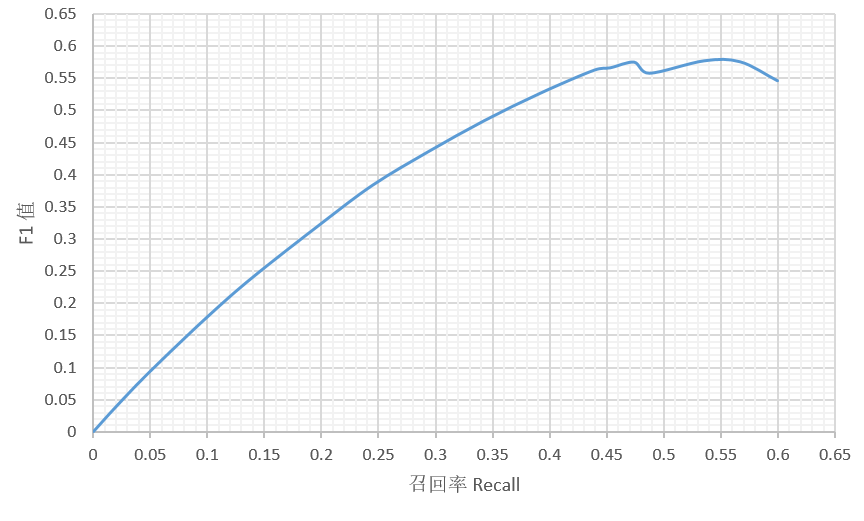
\includegraphics[width=15cm]{performance}
\caption[ZORE 性能图]{ZORE 基于语料库“燃规3”的 F1 值}\label{fig:performance}
\end{figure}

评价程序数据生成的算法性能图 ~\ref{fig:performance} 以 F1 值作为 ZORE 算法综合性能的评价,下表为基于运行评价程序所得出的数据。可以看出,随着词性过滤阈值 $t^{sem}$ 的下降,算法的召回率 Recall 不断提高,而精确率 Precision 却在不断下降,对算法的综合性能衡量指标 F1 值则上下浮动,大体上呈现一种多次函数的模式。

图 ~\ref{fig:performance} 显示了在不同的召回率下 ZORE 在“燃规3”数据集中的表现。体现了先前提及的对召回率 Recall 与精确度 Precision 的平衡性权衡,即 F1 的值先是随着召回率 Recall 的增加而增加,到达极大值后开始下降,则选择 F1 拥有极大值处的召回率 Recall 值可以获得当前语料库下 ZORE 算法的最佳综合性能表现。

同时,以另一种开放式关系抽取算法 DPM\citep{liyang2016} 来与 ZORE 的性能进行比较。二者之间最大的区别就是 DPM 算法增加了对于兼类词的探测和处理,使词性标注出现错误的概率降低,从而提升关系抽取的精确性 Precision,其余处理部分大体相同,也可称之为 ZORE 的兼类词处理版本。

\begin{figure}[h!]
\centering
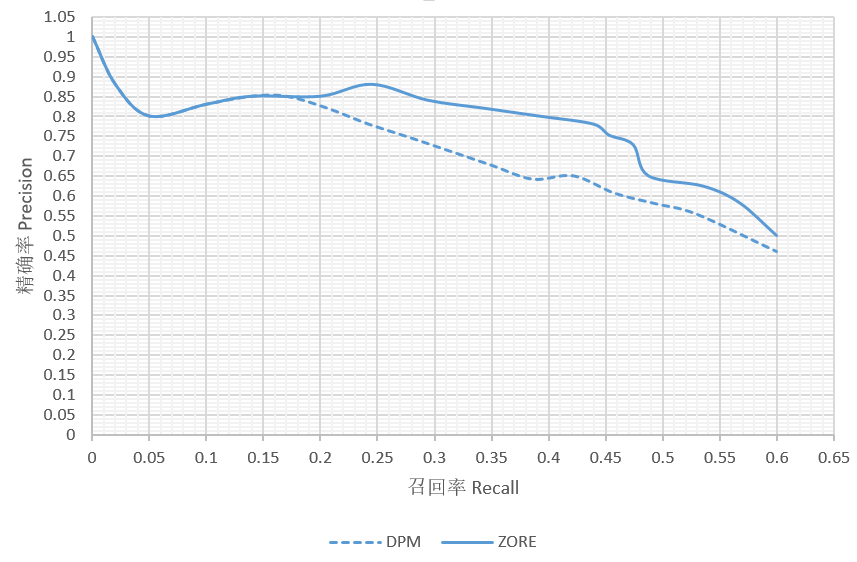
\includegraphics[width=15cm]{compare}
\caption{ZORE 与 DPM 的 P-R 曲线对比}\label{fig:compare}
\end{figure}

\begin{longtable}{|c|c|c|c|}
% 首页表头
\caption[DPM 性能数据]{DPM 运行于语料库“燃规3”上的性能数据} \label{tab:DPMperformance} \\
\toprule[1.5pt]
 召回率 & F1 值 & 精确率 & $t^{sem}$\\
\midrule[1pt]
\endfirsthead
% 续页表头
\caption[]{DPM 运行于语料库“燃规3”上的性能数据(续)} \\
\toprule[1.5pt]
 召回率 & F1 值 & 精确率 & $t^{sem}$\\
\midrule[1pt]
\endhead
% 首页表尾
\hline
\multicolumn{4}{r}{\small 续下页}
\endfoot
% 续页表尾
\bottomrule[1.5pt]
\endlastfoot
0	&	0	&	1	&	19\\
\hline
0.02	&	0.039111111	&	0.88	&	18\\
\hline
0.05	&	0.094117647	&	0.8	&	17\\
\hline
0.1	&	0.178494624	&	0.83	&	16\\
\hline
0.14	&	0.24040404	&	0.85	&	15\\
\hline
0.17	&	0.283333333	&	0.85	&	14\\
\hline
0.206	&	0.329278752	&	0.82	&	13\\
\hline
0.242	&	0.369393346	&	0.78	&	12\\
\hline
0.278	&	0.405152895	&	0.746666667	&	11\\
\hline
0.314	&	0.435742606	&	0.711666667	&	10\\
\hline
0.35	&	0.461363636	&	0.676666667	&	9\\
\hline
0.386	&	0.48203049	&	0.641666667	&	8\\
\hline
0.422	&	0.511753731	&	0.65	&	7\\
\hline
0.458	&	0.521830254	&	0.606333333	&	6\\
\hline
0.494	&	0.533556797	&	0.58	&	5\\
\hline
0.53	&	0.5415749	&	0.553666667	&	4\\
\hline
0.5931	&	0.520754717	&	0.464	&	3\\
\end{longtable}

\begin{figure}[h!]
\centering
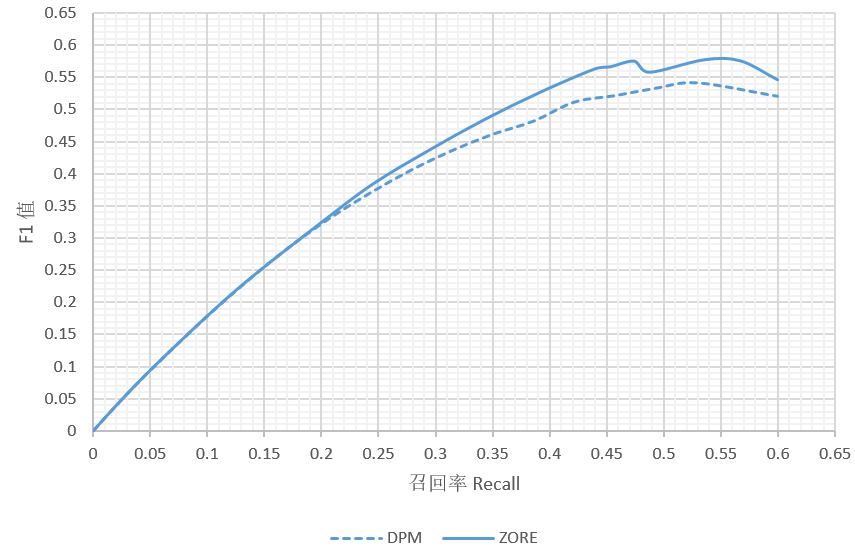
\includegraphics[width=15cm]{comparef}
\caption{ZORE 与 DPM 的 F1 值对比}\label{fig:comparef}
\end{figure}

为了对比的公正客观性,也以“燃规3”作为其语料库进行处理。图 ~\ref{fig:compare} 即为二者运行于同一语料库上的对比图表,可见在特定召回率 Recall 区间上,DPM 精确度 Precision 劣于 ZORE 算法,推断是是由于该语料库是法规,文本结构较为碎片化,以上下文环境进行分析的兼类词处理难以顺利工作导致的。

二者的 P-R 曲线都是体现了精确率 Precision 与召回率 Recall 成反比关系。以及二者之间 F1 值在各种召回率 Recall 下的表现,如图 ~\ref{fig:comparef} 所示,可以看出 DPM 与 ZORE 之间的 F1 值区别并不大,所以可以推断,仅仅增加了对于兼类词处理模块的改进 ZORE 算法得到的 DPM 并没有本质上的提升,即缺少对兼类词处理不是 ZORE 算法提升性能所遇到的瓶颈。

本文经过 ZORE 对语料库“燃规3”进行关系抽取之后,得到了“type\_new.txt”这个所提取出的关系模式统计文件,当中包括了 30 个关系模式及其在训练数据集当中出现的频次和在当前所处理的语料库中出现的频次,以 20 次作为高频出现的阈值,这 30 个关系模式中存在 3 个高频关系模式,分别为:Pattern(nsubj-m(Dn), Pred[de], dobj-n(Di)),22 次;Pattern(nsubj-n(A0), Pred[de], dobj-n(A1)),38 次;Pattern(nsubj-q(Dn), Pred[de], dobj-n(Di)),21 次。很显然,这三个模式都是以“的”为谓词短语的关系模式,与现实生活里的经验符合:由“的”构成的三元组关系模式占正常生活里中文语境下的文本的大多数。

\section{错误分析}
在观察了输出的结果文件后,对不正确的提取(由于精确度的损失)与遗漏的正确的关系(由于召回的损失)进行了统计,得出约 $40\%$ 的遗漏关系是因为语义模式的最低频率限制所导致,而对于语义模式最低频率的限制则是用来平衡召回率与精确率的。

还有一个主要的错误原因是由于解析错误导致的对谓词短语的错误鉴别,带来了全部错误中约 $37\%$ 的报错。也存在由于自然语言处理工具所导致的错误,有分词、依存句法、词性标记等方面产生的错误,例如图 ~\ref{fig:result} 中 argument id = 0 的论元应为 “建、构筑物”而不是“、构筑物”。

这个分词错误也导致了 ZORE 对 id = 326 的句子进行关系抽取时产生了遗漏,关系(设有液化天然气工艺设备,的,建、构筑物)应该在分词正确的前提下被抽取出来。分词错误还会导致对论元的归纳错误,进而影响对 feature 匹配的计量,无法对当前进行分析的句子通过所符合的 feature 数量进行正确的置信度计算,最终影响关系的置信度权重值,使 $Logistic$ 回归分类器无法以当初所预计的工作效果继续工作。

在进行关系提取的过程中也存在选择了错误的模式进行抽取以及未找到可以进行匹配的模式的问题,举个例子,“为使城镇燃气工程设计符合安全生产、保证供应、经济合理和保护环境的要求,制定本规范。”这个句子就未搜索到可以和他匹配的模式进行关系抽取,进而遗漏了(使城镇燃气工程设计,符合,安全生产、保证供应、经济合理和保护环境的要求,制定,本规范),(安全生产、保证供应、经济合理和保护环境,的,要求)这两个关系。

分析结果表明,ZORE 的提取所得到的模式精确率与全面率还有待提升,另外,经过分析可以得出:自然语言处理的工具的性能是提升开放式关系提取算法的瓶颈,句法分析的提升和更加全面且精确的分词系统有很大的可能性让开放式关系抽取也随之进步,所以进行深入研究关于自然语言的处理也是提升开放式关系抽取系统效率的方法之一。亦可追加关系元组进入关系知识库当中,以增加匹配面,故也可对知识库的应用加以研究。

\section{本章小结}
这一章完成了基于特定语料库的算法运行,并对算法的运行结果进行了分析,根据经典的对开放式关系抽取系统的评价标准 P-R 图衡量了算法 ZORE 的综合性能,并验证了词性标签阈值 $t^{sem}$ 对 P-R 图的影响、P-R 二者之间成反比的关系与其权衡。

将 ZORE 与其拥有兼类词处理版本的算法 DPM 进行对比,分析并得出了兼类词处理对于中文开放式关系抽取系统的精确率 Precision 的影响推论。

对于 ZORE 系统的改进,提出了加强系统所使用自然语言处理模块的性能,包括其分词、词性标注、依存句法分析的准确性提高;向关系知识库中追加新的关系元组以增大匹配面;添加对模式进行筛选的算法从而提高对其鉴别的准确性和其对语料库的覆盖率等未来研究方向的设想。
% \chapter{总结与展望}
% 本文调研了当前对于中文的开放式关系抽取的研究现状,开放式关系抽取系统通过识别任意句子中的关系短语和相关参数,从文本中提取关系元组,而不需要预先指定的词汇表。然而,现代最先进的开放式关系抽取系统如 REVERB 和 WOE 有着两个共同的缺点,它们仅提取由动词介导的关系,并且它们忽略上下文,从而提取出了不正确的关系元组。首先,ZORE 通过提取由名词,形容词等介导的关系来实现较高的效率。 第二,上下文分析步骤通过在提取中包括句子中的上下文信息来提高精度,通过识别由名词和形容词介导的关系来扩展开放式关系抽取系统的句法范围。

% 最近已经提出了大量的开放关系提取方法,涵盖了从“浅”(例如,词性标签 POS)到“深”(例如,语义角色标签-SRL)的广泛的NLP机制。 一个重要的问题是NLP深度(和相关的计算成本)与有效性之间的权衡。

% 我们的实验发现,对于某些关系,开放式关系抽取的精确率可能不足。通过分析提取的上下文环境,开放式关系抽取系统能够识别许多和上下文有关的关系,但是是假设的或有条件的。 开放式关系抽取系统通过减少这些提取的置信度或通过归因和分类修饰符的形式将提取中的附加上下文相关联来提高精度。
\bibliography{bib/tex}

\end{document}
